\documentclass{article}
\usepackage[utf8]{inputenc}
\usepackage{relsize}

\title{Graph-based component diagram\\ {\smaller Formal Report}}

\author{Ahmed Yehia}
\date{April 2013}

\usepackage{natbib}
\usepackage{graphicx}

\begin{document}

\maketitle


\section{Abstract}
Cadena-e is based on a component oriented programming paradigm.
Components are software artifacts that form the primary building blocks
of a system (comparable to objects in object oriented programming), they
are defined by their interfaces and can be easily plugged together or inter-
changed. Component diagrams specify how various components interact
within a larger system. The structural modeling tools in Cadena-e should
allow for designing component diagram styles, creating components, and
assembling the components into scenarios.
In this project, we will use the graph editing features in eclipse to build
a three tier component graph creation and editing feature for Cadena-e.



\section{Introduction}
Meta modeling is a wide-spread technique to define visual languages, using the UML The meta modeling approach has several advantages, one of them being that a visual meta model allows a quick grasp of the concepts being defined. Further,The meta modeling approach is also beneficial when it comes to defining complex modeling languages.A component diagram depicts how components are wired together to form larger components and or software systems. They are used to illustrate the structure of arbitrarily complex systems.

{Karsten Ehrig, Jochen M. K ̈uster, Gabriele Taentzer, and Jessica Winkelmann}



\section{Research on github}

I started research on Git Respositorie plug-in ,I learned how to use the plugin,and started to install the plug-in in my Eclipse and pull the Cadana project,started making my own folder and sharing my files with my colleges. 

\begin{figure}[htp]
\centering
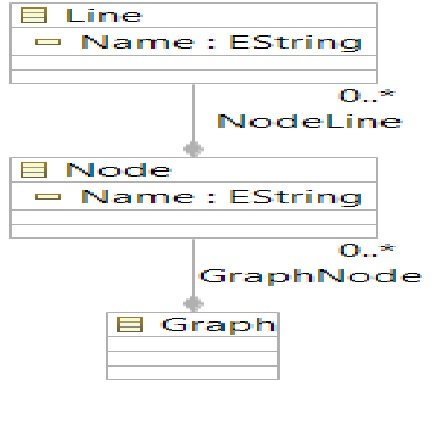
\includegraphics[width=1\linewidth]{Ecore diagram.jpg}
\caption{The Ecore diagram}
\label{threadsVsSync}
\end{figure}

See \figurename~\ref{threadsVsSync}

\section{Eclipse plug-in developant}

Started research about eclipse plug-in,I learned how to install a plug-in and use plug-in and also to create a plug-in from Eclipse marketplace.

\section{Research eclipse graphical editing}
Started researching on graphical tool,learning about different tools and different plug-in i started with Eclipse Modeling Framework is an Eclipse-based modeling framework and code generation facility for building tools and other applications based on a structured data model. their are many plug-ins that use things like EMF First, I started to resarch Eclipse Zest plug-in Zest is Eclipse Zest is a visualization toolkit for graphs.

But than I concluded that it can not be used with meta-modeling ,It is just a drawing tool and than started to research emf2gv (EMF to Graphviz) this tools allows the use to generate a grapical representation of models. I installed the tool in my Eclipse,and started testing the plug-in.It was hard to do the Models with this tool.
I started searching for a new tool than I found the GMF,GMF is a generative components and runtime infrastructures for developing graphical editors based on EMF.The GMF Tooling provides a model-driven approach to generating graphical editors,First I had to make my data model,The medol represents the data that i work with also known with domain model.
Once the EMF model is done it can generate the  Java  classes from this model,The model uses XML to produce the model definition.I Install EMF via the Eclipse Update manager then Selected Modeling and EMF - Eclipse Modeling Framework SDK also GMF Runtime 1.5.x with GMF Tooling.
I Created a new project File → New → other→ Graphical Modeling Framework → Graphical editor Project .
Under model right click new Ecore diagram,than started making my classes(eclasses)(Graph,Node,Line).
Node class contains one EAttribute Name type EString,Line class contains one EAttribute Name type EString.Graph class.
I created two EReferences the first one is GraphNode which says that i graph has many nodes.The other is NodeLine.One node has many lines.
After making the model initialze the Ecore diagram.Than i started with GMF Dashboard to generate the diagram.First i derived domain Gen Model than Graphical Def model than the tooling Def model than combine the two models creating the mapping model,Using the transform to generate 
the diagram editor.

\section{Research on style tier}
Started research on the style tier.The most Important tool in the style tier is CALM (www.cadena.projects.cis.ksu.edu/calm) is an
architecture description language that enables strongly
typed modeling of platforms,\cite{Adam Childs, Jesse Greenwald, Georg Jung, Matthew Hoosier, and John Hatcliff}


\begin{figure}[htp]
\centering
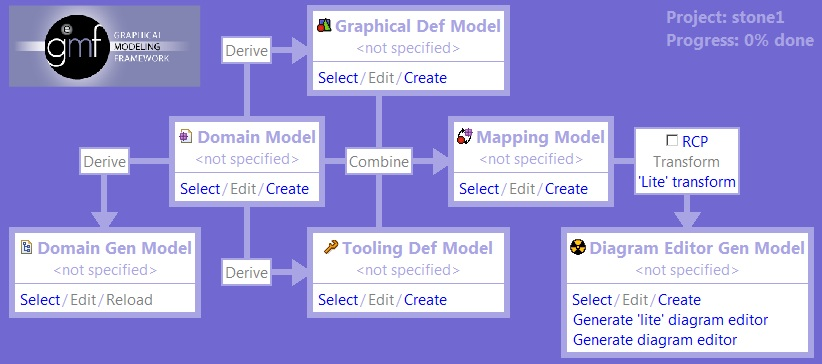
\includegraphics[width=1\linewidth]{GMF Dashboard.jpg}
\caption{The Dashboard}
\label{threadsVsSync}
\end{figure}



\bibliographystyle{plain}
\bibliography{references}
\end{document}
